% Options for packages loaded elsewhere
\PassOptionsToPackage{unicode}{hyperref}
\PassOptionsToPackage{hyphens}{url}
%
\documentclass[
  english,
  man]{apa6}
\usepackage{amsmath,amssymb}
\usepackage{lmodern}
\usepackage{ifxetex,ifluatex}
\ifnum 0\ifxetex 1\fi\ifluatex 1\fi=0 % if pdftex
  \usepackage[T1]{fontenc}
  \usepackage[utf8]{inputenc}
  \usepackage{textcomp} % provide euro and other symbols
\else % if luatex or xetex
  \usepackage{unicode-math}
  \defaultfontfeatures{Scale=MatchLowercase}
  \defaultfontfeatures[\rmfamily]{Ligatures=TeX,Scale=1}
\fi
% Use upquote if available, for straight quotes in verbatim environments
\IfFileExists{upquote.sty}{\usepackage{upquote}}{}
\IfFileExists{microtype.sty}{% use microtype if available
  \usepackage[]{microtype}
  \UseMicrotypeSet[protrusion]{basicmath} % disable protrusion for tt fonts
}{}
\makeatletter
\@ifundefined{KOMAClassName}{% if non-KOMA class
  \IfFileExists{parskip.sty}{%
    \usepackage{parskip}
  }{% else
    \setlength{\parindent}{0pt}
    \setlength{\parskip}{6pt plus 2pt minus 1pt}}
}{% if KOMA class
  \KOMAoptions{parskip=half}}
\makeatother
\usepackage{xcolor}
\IfFileExists{xurl.sty}{\usepackage{xurl}}{} % add URL line breaks if available
\IfFileExists{bookmark.sty}{\usepackage{bookmark}}{\usepackage{hyperref}}
\hypersetup{
  pdftitle={Job Demands-Resources model components through the lens of O*NET classifications},
  pdfauthor={Alicia Stachowski1, Renata Garcia Prieto Palacios Roji2, \& John Kulas2},
  pdflang={en-EN},
  pdfkeywords={keywords},
  hidelinks,
  pdfcreator={LaTeX via pandoc}}
\urlstyle{same} % disable monospaced font for URLs
\usepackage{graphicx}
\makeatletter
\def\maxwidth{\ifdim\Gin@nat@width>\linewidth\linewidth\else\Gin@nat@width\fi}
\def\maxheight{\ifdim\Gin@nat@height>\textheight\textheight\else\Gin@nat@height\fi}
\makeatother
% Scale images if necessary, so that they will not overflow the page
% margins by default, and it is still possible to overwrite the defaults
% using explicit options in \includegraphics[width, height, ...]{}
\setkeys{Gin}{width=\maxwidth,height=\maxheight,keepaspectratio}
% Set default figure placement to htbp
\makeatletter
\def\fps@figure{htbp}
\makeatother
\setlength{\emergencystretch}{3em} % prevent overfull lines
\providecommand{\tightlist}{%
  \setlength{\itemsep}{0pt}\setlength{\parskip}{0pt}}
\setcounter{secnumdepth}{-\maxdimen} % remove section numbering
% Make \paragraph and \subparagraph free-standing
\ifx\paragraph\undefined\else
  \let\oldparagraph\paragraph
  \renewcommand{\paragraph}[1]{\oldparagraph{#1}\mbox{}}
\fi
\ifx\subparagraph\undefined\else
  \let\oldsubparagraph\subparagraph
  \renewcommand{\subparagraph}[1]{\oldsubparagraph{#1}\mbox{}}
\fi
% Manuscript styling
\usepackage{upgreek}
\captionsetup{font=singlespacing,justification=justified}

% Table formatting
\usepackage{longtable}
\usepackage{lscape}
% \usepackage[counterclockwise]{rotating}   % Landscape page setup for large tables
\usepackage{multirow}		% Table styling
\usepackage{tabularx}		% Control Column width
\usepackage[flushleft]{threeparttable}	% Allows for three part tables with a specified notes section
\usepackage{threeparttablex}            % Lets threeparttable work with longtable

% Create new environments so endfloat can handle them
% \newenvironment{ltable}
%   {\begin{landscape}\begin{center}\begin{threeparttable}}
%   {\end{threeparttable}\end{center}\end{landscape}}
\newenvironment{lltable}{\begin{landscape}\begin{center}\begin{ThreePartTable}}{\end{ThreePartTable}\end{center}\end{landscape}}

% Enables adjusting longtable caption width to table width
% Solution found at http://golatex.de/longtable-mit-caption-so-breit-wie-die-tabelle-t15767.html
\makeatletter
\newcommand\LastLTentrywidth{1em}
\newlength\longtablewidth
\setlength{\longtablewidth}{1in}
\newcommand{\getlongtablewidth}{\begingroup \ifcsname LT@\roman{LT@tables}\endcsname \global\longtablewidth=0pt \renewcommand{\LT@entry}[2]{\global\advance\longtablewidth by ##2\relax\gdef\LastLTentrywidth{##2}}\@nameuse{LT@\roman{LT@tables}} \fi \endgroup}

% \setlength{\parindent}{0.5in}
% \setlength{\parskip}{0pt plus 0pt minus 0pt}

% Overwrite redefinition of paragraph and subparagraph by the default LaTeX template
% See https://github.com/crsh/papaja/issues/292
\makeatletter
\renewcommand{\paragraph}{\@startsection{paragraph}{4}{\parindent}%
  {0\baselineskip \@plus 0.2ex \@minus 0.2ex}%
  {-1em}%
  {\normalfont\normalsize\bfseries\itshape\typesectitle}}

\renewcommand{\subparagraph}[1]{\@startsection{subparagraph}{5}{1em}%
  {0\baselineskip \@plus 0.2ex \@minus 0.2ex}%
  {-\z@\relax}%
  {\normalfont\normalsize\itshape\hspace{\parindent}{#1}\textit{\addperi}}{\relax}}
\makeatother

% \usepackage{etoolbox}
\makeatletter
\patchcmd{\HyOrg@maketitle}
  {\section{\normalfont\normalsize\abstractname}}
  {\section*{\normalfont\normalsize\abstractname}}
  {}{\typeout{Failed to patch abstract.}}
\patchcmd{\HyOrg@maketitle}
  {\section{\protect\normalfont{\@title}}}
  {\section*{\protect\normalfont{\@title}}}
  {}{\typeout{Failed to patch title.}}
\makeatother
\shorttitle{O*NET JD-R}
\keywords{keywords\newline\indent Word count: X}
\DeclareDelayedFloatFlavor{ThreePartTable}{table}
\DeclareDelayedFloatFlavor{lltable}{table}
\DeclareDelayedFloatFlavor*{longtable}{table}
\makeatletter
\renewcommand{\efloat@iwrite}[1]{\immediate\expandafter\protected@write\csname efloat@post#1\endcsname{}}
\makeatother
\usepackage{csquotes}
\ifxetex
  % Load polyglossia as late as possible: uses bidi with RTL langages (e.g. Hebrew, Arabic)
  \usepackage{polyglossia}
  \setmainlanguage[]{english}
\else
  \usepackage[main=english]{babel}
% get rid of language-specific shorthands (see #6817):
\let\LanguageShortHands\languageshorthands
\def\languageshorthands#1{}
\fi
\ifluatex
  \usepackage{selnolig}  % disable illegal ligatures
\fi
\newlength{\cslhangindent}
\setlength{\cslhangindent}{1.5em}
\newlength{\csllabelwidth}
\setlength{\csllabelwidth}{3em}
\newenvironment{CSLReferences}[2] % #1 hanging-ident, #2 entry spacing
 {% don't indent paragraphs
  \setlength{\parindent}{0pt}
  % turn on hanging indent if param 1 is 1
  \ifodd #1 \everypar{\setlength{\hangindent}{\cslhangindent}}\ignorespaces\fi
  % set entry spacing
  \ifnum #2 > 0
  \setlength{\parskip}{#2\baselineskip}
  \fi
 }%
 {}
\usepackage{calc}
\newcommand{\CSLBlock}[1]{#1\hfill\break}
\newcommand{\CSLLeftMargin}[1]{\parbox[t]{\csllabelwidth}{#1}}
\newcommand{\CSLRightInline}[1]{\parbox[t]{\linewidth - \csllabelwidth}{#1}\break}
\newcommand{\CSLIndent}[1]{\hspace{\cslhangindent}#1}

\title{Job Demands-Resources model components through the lens of O*NET classifications}
\author{Alicia Stachowski\textsuperscript{1}, Renata Garcia Prieto Palacios Roji\textsuperscript{2}, \& John Kulas\textsuperscript{2}}
\date{}


\authornote{

Correspondence concerning this article should be addressed to Alicia Stachowski, Menomenie, WI. E-mail: \href{mailto:stachowskia@uwstout.edu}{\nolinkurl{stachowskia@uwstout.edu}}

}

\affiliation{\vspace{0.5cm}\textsuperscript{1} University of Wisconsin - Stout\\\textsuperscript{2} Montclair State University}

\abstract{
O*NET work characteristics were rated in terms of relevance, perception as a demand, and perception as a resource. All the results of this current study match the stress-appraisal stuff. Next steps: 1) discuss results within stress-appraisal framework (Lazarus \& Bookman), 2) different literature on challenge and hindrance demands. Job Demands Resources theory that says resources and demands are relatively universal is NOT consistent with these findings. JDR neglects the other 2 literatures. Analytically pull O*Net descriptors that reflect universal demands/resources (e.g., autonomy) and see how much variability there is on those. Maybe forget about cross-walk thing. May actually want to start with this: \url{https://docs.google.com/spreadsheets/d/1ck-72dQ_c-Pl4Xba9W0r__OYo0znlEnV/edit\#gid=1041061499}.{[}\^{}foot1{]}

We want to also group items by O*NET categories so there's not so many (that makes ANOVAs more viable)
}



\begin{document}
\maketitle

Research on the job demands-resources model (Demerouti et al., 2001) and later job demands-resources theory (A. B. Bakker \& Demerouti, 2017) highlight the importance of work characteristics on the experience of motivation and strain, which clearly have an impact on job performance. In light of some of the recent debate surrounding the challenge-hindrance stressor framework (e.g., Mazzola \& Disselhorst, 2019), we extend this critical research to that of the subjective distinction between challenge and hindrance demands (and resource) in the workplace, and how they relate to two important organizational outcomes: engagement and stress. Prior to presenting the current study in detail, we provide a brief overview of the relevant theories and relevant empirical work on this topic.

\hypertarget{the-job-demands-resources-theory}{%
\subsection{The Job demands-Resources Theory}\label{the-job-demands-resources-theory}}

The overarching context for this study is that of the job demands-resources theory, which is an expansion of the well-studied job demands-resources model (Demerouti et al., 2001). One of the major advantages of the job demands-resources theory is that it allows us to model both work environment and job characteristics via job resources and demands. \emph{Resources} include physical, psychological, social, or organizational aspects of the job that may help an employee achieve work goals, reduce job demands, or promote personal growth and development (Demerouti et al., 2001). In contrast, demands include components of a job that require sustained effort, and as such, produce psychological or physiological strain (e.g., high work pressure is frequently cited as a common demand; Demerouti et al. (2001)).

Cognitively, the perception of an element of one's job as a resource or demand activates one of two distinct processes: either health impairment (resulting from demands) or motivation (resulting from resources) (A. B. Bakker \& Demerouti, 2014). Pertinent to the current study, demanding job characteristics are frequently often associated with negative outcomes (e.g., A. Bakker et al., 2003), whereas job characteristics deemed resources have been associated with positive organizational outcomes like engagement and motivation (A. B. Bakker et al., 2007).

\hypertarget{the-essential-role-of-appraisal}{%
\subsection{The Essential Role of Appraisal}\label{the-essential-role-of-appraisal}}

As implied in the last paragraph, job context and characteristics are ``assigned'' or appraised as demands or resources. Although some research on job demands in particular is based on apriori classifications of demands (Searle \& Auton, 2015), the classification of a work characteristic as a demand or resource is largely subjective by nature (e.g., an employee could most certainly perceive being a public figure as a resource or as a demand. The stress process speaks to how such individual difference in appraisal is possible. Lazarus and Folkman (1984) presented the transactional theory of stress and coping, which states that people cognitively appraise stimuli in their environments on a continuous basis. Via this process, meaning is assigned to stimuli -- if appraised as threatening, challenging, or possibly harmful, the resulting emotional distress initiates coping. The cycle of appraisal then continues based on the action to cope with the stressor (Lazarus \& Folkman, 1984).

\hypertarget{the-challenge-hindrance-stressor-framework}{%
\subsection{The Challenge-hindrance Stressor Framework}\label{the-challenge-hindrance-stressor-framework}}

Although there is a tendency to attach a negative connotation to the word ``stress,'' Selye (1936) defined stress as a response to change, which is quite non-specific. We return to the employed public figure for this next section. It is quite probable that two employees would be called upon to serve as a spokesperson for their organization in a time of need. One may appraise the circumstance as an opportunity to positively influence others, while the other may plausibly feel paralyzed by the task. In fact, A. B. Bakker and Demerouti (2017) call attention to different types of demands in their recent review of, and future directions, for work on the job-demands resources theory. The challenge-hindrance stressor framework suggests that the way we understand reactions to stressors requires consideration of how people feel about a given stressor (Cavanaugh et al. (2000)). Cavanaugh et al. (2000) delineated between two forms of demands -- that of \emph{challenge} and \emph{hindrance} demands. Challenge demands promote mastery, personal growth, and future gains -- these stressors should lead to coping strategies that facilitate achievement. Stressors like time pressure and responsibility are considered challenge stressors/demands. hindrance demands, in contrast, inhibit growth, learning and goal achievement. Hindrance stressors (e.g., role conflict, role ambiguity, politics) are associated with negative job behaviors and attitudes. This particular distinction between challenges and hindrances has been of value in determining what demands are related to various outcomes, whereby challenge stressors are typically associated with positive outcomes, and hindrance stressors, negative outcomes (e.g., Cavanaugh et al. (2000)).

However, one of the key questions we need to ask as researchers pertains to the very basic consideration of appraisals. In fact, this is one of several issues raised by @ mazzola2019should in a recent review and meta-analysis of this framework. These authors cited the apriori assignment to stressors as a challenge or hindrance as a flawed assumption, suggesting that stressors are more likely to be a combination of both -- challenge and hindrance appraisals. LePine (2022), in a rebuttal to the @ mazzola2019should criticism, while acknowledging that the original challenge-hindrance stressor framework was based on the assertion that people tend to appraise specific work stressors ad challenges and other demands, noted that the appraisals likely served as a mediator.

We next consider the empirical evidence on this topic. The first obvious question is whether people perceive demands as challenges vs.~hindrances, or whether all demands are under a larger ``demands'' category. Evidence suggests the employees do, in fact, distinguish between challenge and hindrance stressors (e.g., A. B. Bakker \& Sanz-Vergel, 2013; Gerich, 2017; Webster et al., 2011). For example, A. B. Bakker and Sanz-Vergel (2013) found that perceived work pressure as a hindrance demand, and emotional demands as more of a challenge demand. Webster et al. (2011) approached this question with three common workplace demands: workload, role ambiguity, and role conflict. They found while that each could be appraised primarily as challenges or hindrances demands, they could also simultaneously be perceived as being both a challenge and hindrance to different degrees.

While their study did include resources, it nonetheless points to the possibility that demands might be differentially appraised and related to outcomes (e.g., Podsakoff et al., 2007). The challenge-hindrance framework has, in fact, been associated with a wide variety of organizational outcomes ranging from affective variables like job satisfaction, to motivation, performance, and well-being. A sampling of variables and relationships are described below to provide a sense of scope of the work that has been on this topic. For example, Cavanaugh et al. (2000), in a study of managers, found that challenge demands were positively related to job satisfaction and negatively related to job search behaviors, while hindrance demands demonstrated the opposite pattern. In contrast, Abbas and Raja (2019) found that challenge and hindrance stressors were \emph{both} positively related to strain and turnover intentions. We also have some evidence that challenge-hindrance appraisals are related to engagement in the expected direction whereby hindrance appraisals are negatively associated with engagement and challenge appraisals are positively associated with it (Crawford et al., 2010). Challenge and hindrance appraisals have also been shown to relate to citizenship and counterproductive performance, although indirectly via emotions like anxiety (Rodell \& Judge, 2009). Lastly, Gerich (2017) concluded that employee well-being was also, in part, explained by appraised challenge or hindrance demands such that working conditions of time pressure, qualitative demands, responsibility, and interruptions, were partially mediated by challenge and hindrance demands.

We even have sufficient evidence to explore outcomes associated with challenge and hindrance stressors meta-analytically at this point. Podsakoff et al. (2007) supported the original assertion of Cavanaugh et al. (2000) with regard to work outcomes such that challenge stressors were positively related to job satisfaction and organizational commitment, and negatively related to both turnover intentions and actual turnover. The opposite pattern of relationship was observed for hindrance stressors. @ kim2020thriving, similarly, found evidence for the differential results via challenge and hindrance appraisals

\hypertarget{onet-resource}{%
\subsection{O*Net Resource}\label{onet-resource}}

Originally, the Advisory Panel for the Dictionary of Occupational Titles recommended a system that would ``\ldots promote the effective education, training, counseling, and employment of the American workforce. It should accomplish its purpose by providing a database system that identifies, defines, classifies, and describes occupations in the economy in an accessible and flexible manner'' (Dictionary of Occupational Titles (US) and Service (1993), p.~6). The result was the now commonly used O*NET. The Occupational Information Network (O*NET; onetonline.org) contains a comprehensive description of occupations (Peterson et al., 2001). This widely accessed database houses hundreds of standardized and occupation-specific descriptors most occupations in the US and these descriptions are continually updated. In fact, there was a call to work with experienced I/O psychologists over the summer to update the content for the \href{https://www.onetonline.org/link/summary/19-3032.00}{Industrial and Organizational Psychologist listing on O*Net}. These data, and the tools provided for free on the website (e.g., Career Exploration Tools, ``My Next Move for Veterans,'' ``My Next Move,'' Toolkit for Business) are frequently used by counselors, students, human resources departments, and researchers to assist potential applicants discover the skills and training they need for the job of their choice. It is also useful to employers by providing them with information with which to craft job descriptions and help employees determine what skills are needed for promotion.

Of greatest interest here are statements taken from O*NET \href{https://www.O*NETonline.org/find/descriptor/result/4.A.1.b.3}{``activity'' and ``context'' classifications} (e.g., items related to information input, interacting with others, physical work conditions, structural job characteristics). One of the first and basic questions is whether or not the categorical examples of ``resources'' and ``demands'' described in the Job Demands-Resources Theory (Demerouti et al., 2001), for example, are generally deemed resources or demands as we objectively define them. The next logical question surrounds how ``universal'' such ratings are. For instance, it is quite possible, given the theoretical and empirical evidence presented above, that there is wide variability in individual appraisal of work activities and context such that some people may rate a given activity as a resource and others a hindrance.

\begin{quote}
Hypothesis 1: Job characteristics differ in variability/stability regarding subjective worker perception as a demand or resource.
\end{quote}

\begin{quote}
Hypothesis 2: Job characteristics are not uniquely categorized as a resource or demand, but rather, some job characteristics are rated highly as both a resource and a demand.
\end{quote}

Add a description here of the exploratory stuff.

\begin{quote}
\emph{Research Question 1}: Are literature-implicated resources consistently rated as job resources?
\end{quote}

\begin{quote}
\emph{Research Question 2}: Are literature-implicated challenges consistently rated as job challenges?
\end{quote}

\begin{quote}
\emph{Research Question 3}: Are literature-implicated hiderances consistently rated as job hindrances?
\end{quote}

\hypertarget{participants}{%
\subsection{Participants}\label{participants}}

Of the 785 Prolific panel individuals who initially accessed the survey link, 112 indicated that they were not interested, had more than 200 missing responses, or had 20 or more identical consecutive sequential responses (Yentes \& Wilhelm, 2021). Applying a further screen regarding attention checks (there were four attention checks embedded throughout, asking respondents to indicate a specific answer) resulted in the retention of 568 respondents who constitute the current SIOP sample. 13.57\% had been in their referent job less than 6 months, 19.20\% between 6 months and a year, 49.12\% between one and five years, 13.27\% between 5 and 10 years, and 4.87\% more than 10 years.

Ages ranged from 18 to 65 with an average of 28.18 years old (SD = 7.53). The survey offered a free-field gender identity category, although the sample predominantly self-identified as female (52.58\%) or male (46.83\%).

\begin{figure}
\centering
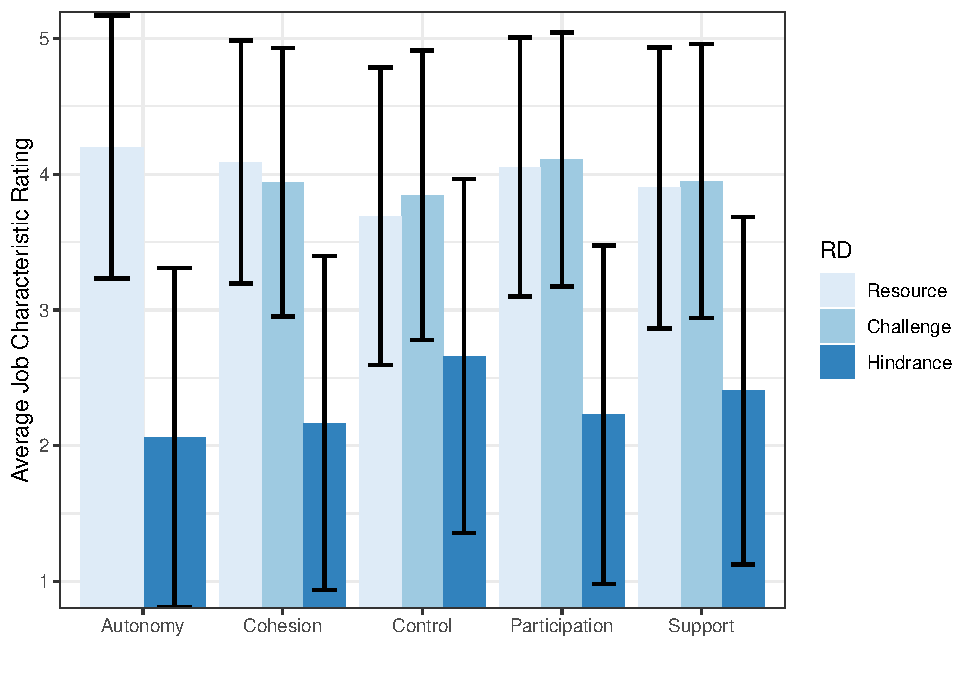
\includegraphics{Submission_files/figure-latex/litresources-1.pdf}
\caption{\label{fig:litresources}Average and standard deviation of O*Net characteristics retained as indicators of Autonomy, Cohesion, Control, Participation, and Supervisor Support.}
\end{figure}

\hypertarget{materials}{%
\subsection{Materials}\label{materials}}

Each free-field job title was placed into one of 14 possible O*NET job families classifications. 60 of these ratings were performed by all 3 author raters, with a resulting Kappa of 0.53 (Landis \& Koch, 1977). We then further collapsed these 14 categories into 8 essentially equal frequency job categories.

\hypertarget{characteristics-demands-and-resources}{%
\subsubsection{Characteristics, Demands, and Resources}\label{characteristics-demands-and-resources}}

We used 98 statements taken from O*NET \href{https://www.O*NETonline.org/find/descriptor/result/4.A.1.b.3}{``activity'' and ``context'' classifications}. We retained 41 ``work activity'' classifications which O*NET groups into categories of ``Information Input'' (5 statements), ``Interacting with Others'' (17 statements), ``Mental Processes'' (10 statements) and ``Work Output'' (9 statements). 57 ``work context'' statements grouped into ``Interpersonal Relationships'' (14 statements), ``Physical Work Conditions'' (30 statements), and ``Structural Job Characteristics'' (13 statements).

These ``descriptors'' often have unique response categories (\href{https://www.O*NETonline.org/find/descriptor/result/4.C.1.c.2}{see here for example}). We retained the O*NET wording to capture characteristics of relevance for each respondent. Subsequent to these self evaluations, each respondent who agreed that the element had \emph{at least some relevance} to their job was also asked to rate that element in terms of, 1) \ldots this aspect of your job is a resource that can be functional in achieving work goals, reduce job demands, or stimulate personal growth/development, 2) \ldots this aspect of your job is a challenge that can promote mastery, personal growth, or future gains, and 3) \ldots this aspect of your job is a hindrance that can inhibit personal growth, learning, and work goal attainment.

\hypertarget{results}{%
\section{Results}\label{results}}

\hypertarget{low-variability-demands-and-resources}{%
\subsection{Low Variability Demands and Resources}\label{low-variability-demands-and-resources}}

The below graphs present the resources, challenges, and hindrances that are \emph{largely agreed on} as indexed by (relatively) low standard deviations.

\begin{quote}
Note. The ``zero'' standard deviations are likely one person, \emph{n}'s should also go on these graphs if they're retained.
\end{quote}

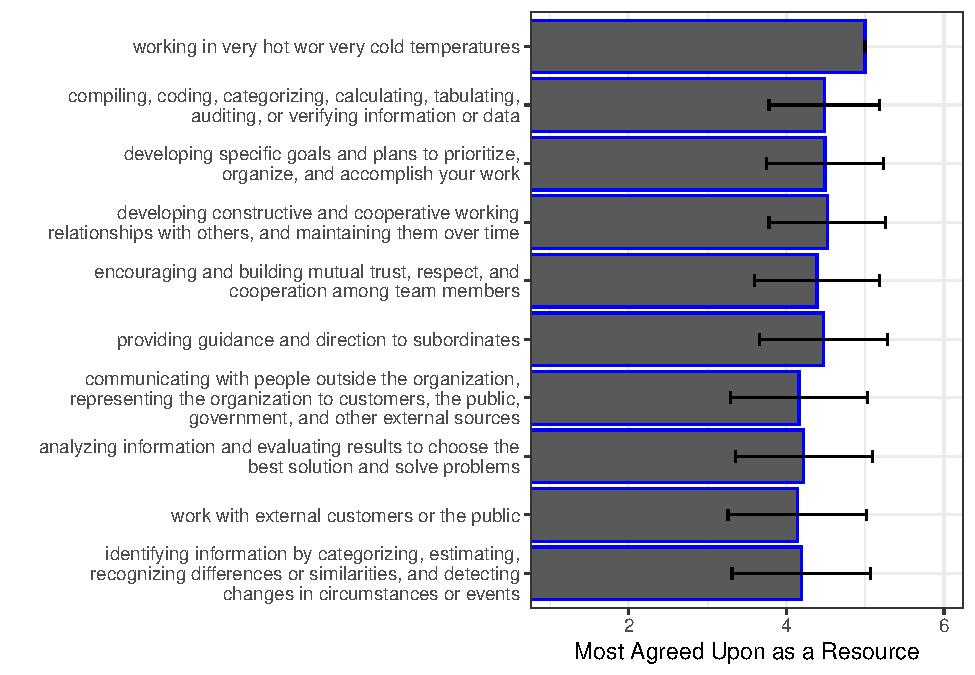
\includegraphics{Submission_files/figure-latex/resourceslowsd-1.pdf}

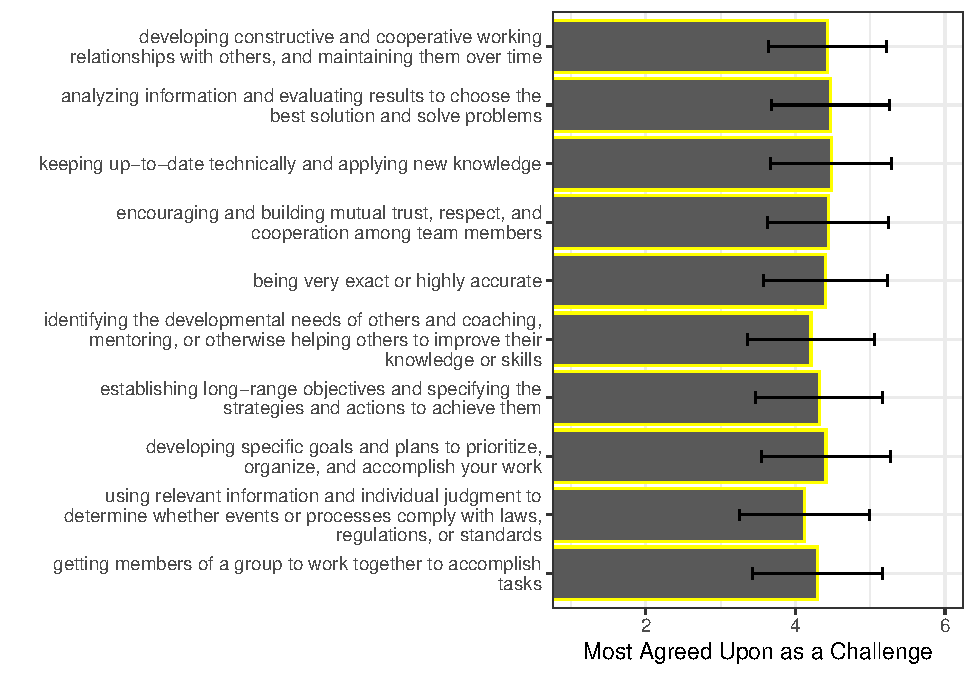
\includegraphics{Submission_files/figure-latex/challengesagree-1.pdf}

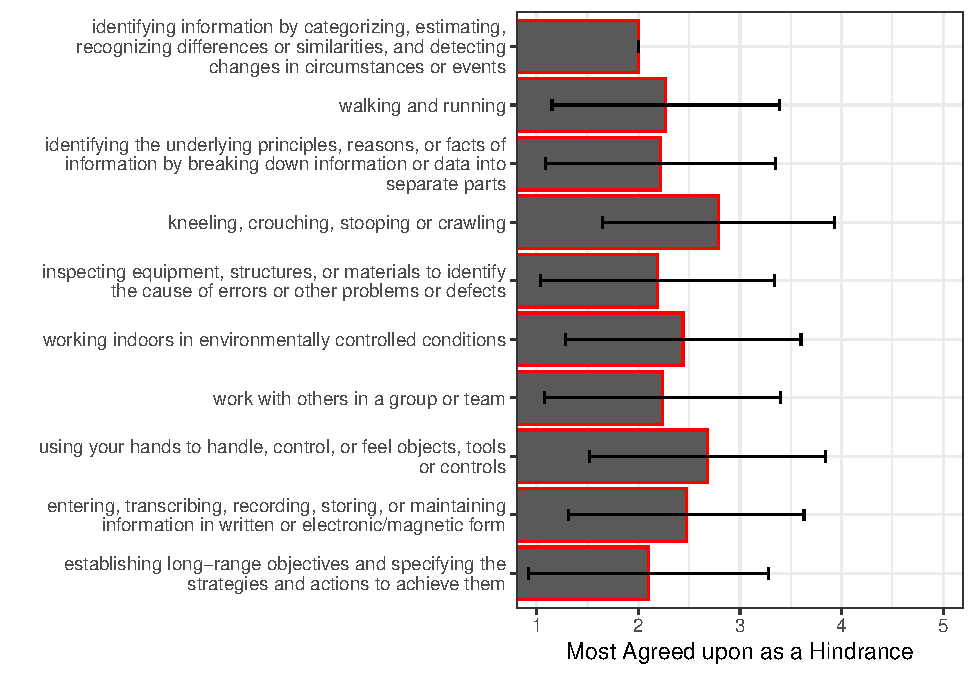
\includegraphics{Submission_files/figure-latex/hindrancesagree-1.pdf}

As can be seen by the graphs, there is considerable disagreement regarding the degree to which job elements are considered \emph{hindrances}, with the 10 elements showing the greatest agreement still ranging in standard deviations from 0 to 1.18. What is widely seen as a resource and challenge tends to be more universally agreed upon (range of lowest 10 resource standard deviations is 0 to 0.88 and the range of lowest 10 challenge standard deviations is 0 to 0.87.

\hypertarget{high-variability-demands-and-resources}{%
\subsection{High Variability Demands and Resources}\label{high-variability-demands-and-resources}}

The below graphs present the resources, challenges, and hindrances that are \emph{largely disagreed on} as indexed by (relatively) high standard deviations (these are the 10 characteristics with the greatest variability in rating).

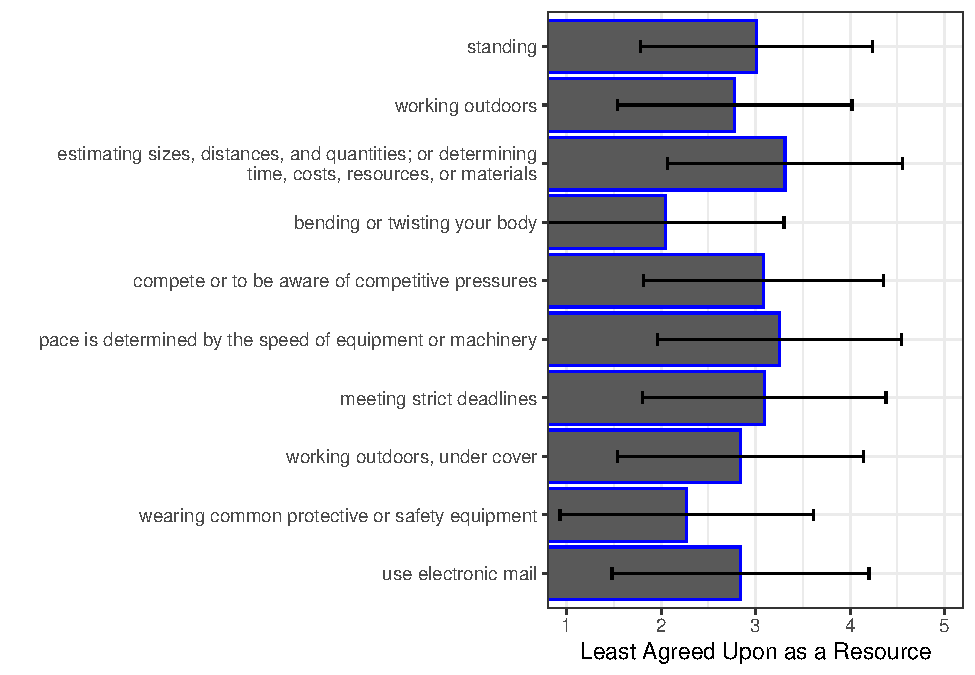
\includegraphics{Submission_files/figure-latex/resourceshisd-1.pdf}

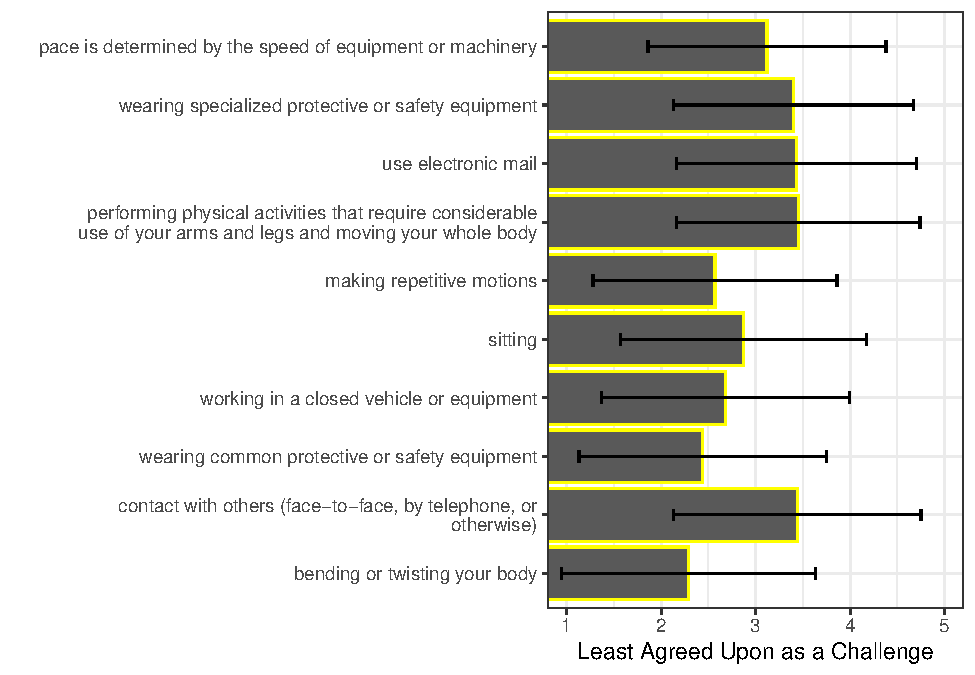
\includegraphics{Submission_files/figure-latex/challengeshighsd-1.pdf}

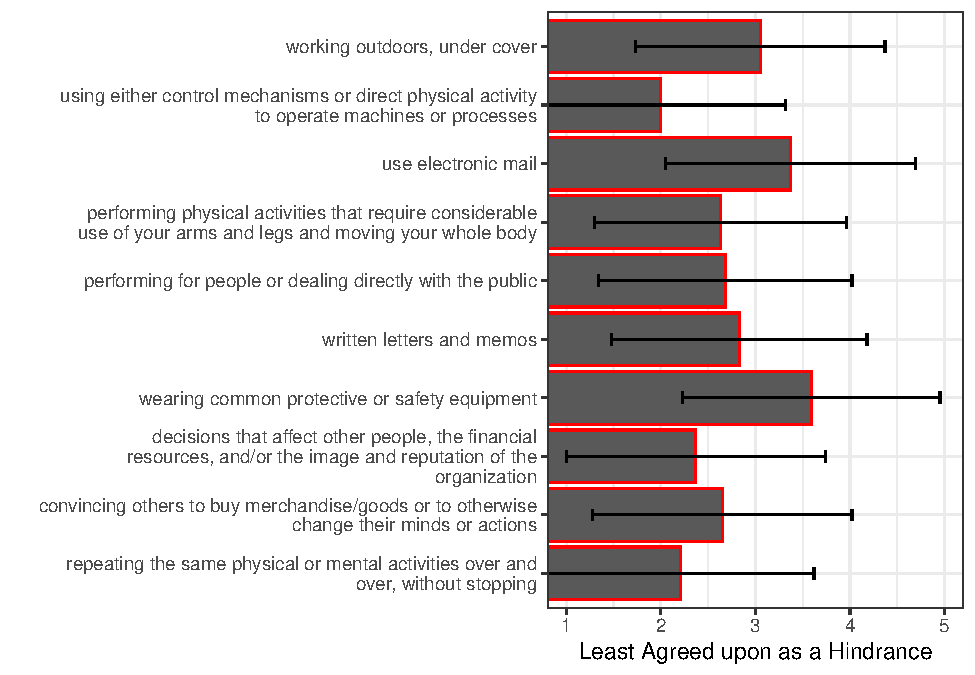
\includegraphics{Submission_files/figure-latex/hindranceshighsd-1.pdf}

\begin{verbatim}
##    Min. 1st Qu.  Median    Mean 3rd Qu.    Max.    NA's 
##   1.000   1.000   2.000   2.185   3.000   5.000       7
\end{verbatim}

\begin{verbatim}
##    Min. 1st Qu.  Median    Mean 3rd Qu.    Max.    NA's 
##   1.000   4.000   4.500   4.202   5.000   5.000       7
\end{verbatim}

\begin{verbatim}
##    Min. 1st Qu.  Median    Mean 3rd Qu.    Max.    NA's 
##   1.000   4.000   4.500   4.205   5.000   5.000       7
\end{verbatim}

\begin{verbatim}
## 
##             Autonomy    Emotional Demands          Job Control 
##                 1704                 1704                 1704 
##             Overwork        Participation Physical Environment 
##                 1704                 1704                 1704 
##    Recipient Contact        Team Cohesion        Time Pressure 
##                 1704                 1704                 1704 
##        Work Pressure 
##                 1704
\end{verbatim}

\begin{figure}
\centering
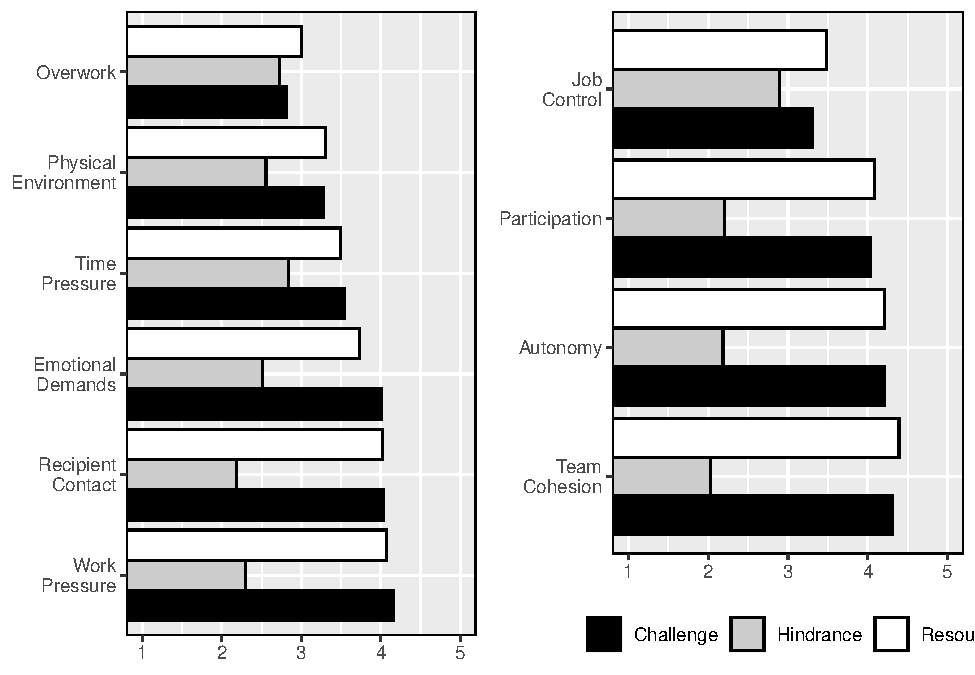
\includegraphics{Submission_files/figure-latex/scalelevelgraphs-1.pdf}
\caption{\label{fig:scalelevelgraphs}Average characteristic rating grouped by literature-implicated categorizations.}
\end{figure}

see Figure \ref{fig:scalelevelgraphs}

\newpage

\hypertarget{references}{%
\section{References}\label{references}}

\begingroup
\setlength{\parindent}{-0.5in}
\setlength{\leftskip}{0.5in}

\hypertarget{refs}{}
\begin{CSLReferences}{1}{0}
\leavevmode\hypertarget{ref-abbas2019challenge}{}%
Abbas, M., \& Raja, U. (2019). Challenge-hindrance stressors and job outcomes: The moderating role of conscientiousness. \emph{Journal of Business and Psychology}, \emph{34}(2), 189--201.

\leavevmode\hypertarget{ref-bakker2014job}{}%
Bakker, A. B., \& Demerouti, E. (2014). Job demands--resources theory. \emph{Wellbeing: A Complete Reference Guide}, 1--28.

\leavevmode\hypertarget{ref-bakker2017job}{}%
Bakker, A. B., \& Demerouti, E. (2017). Job demands--resources theory: Taking stock and looking forward. \emph{Journal of Occupational Health Psychology}, \emph{22}(3), 273.

\leavevmode\hypertarget{ref-bakker2007job}{}%
Bakker, A. B., Hakanen, J. J., Demerouti, E., \& Xanthopoulou, D. (2007). Job resources boost work engagement, particularly when job demands are high. \emph{Journal of Educational Psychology}, \emph{99}(2), 274.

\leavevmode\hypertarget{ref-bakker2013weekly}{}%
Bakker, A. B., \& Sanz-Vergel, A. I. (2013). Weekly work engagement and flourishing: The role of hindrance and challenge job demands. \emph{Journal of Vocational Behavior}, \emph{83}(3), 397--409.

\leavevmode\hypertarget{ref-bakker2003dual}{}%
Bakker, A., Demerouti, E., \& Schaufeli, W. (2003). Dual processes at work in a call centre: An application of the job demands--resources model. \emph{European Journal of Work and Organizational Psychology}, \emph{12}(4), 393--417.

\leavevmode\hypertarget{ref-cavanaugh2000empirical}{}%
Cavanaugh, M. A., Boswell, W. R., Roehling, M. V., \& Boudreau, J. W. (2000). An empirical examination of self-reported work stress among US managers. \emph{Journal of Applied Psychology}, \emph{85}(1), 65.

\leavevmode\hypertarget{ref-crawford2010linking}{}%
Crawford, E. R., LePine, J. A., \& Rich, B. L. (2010). Linking job demands and resources to employee engagement and burnout: A theoretical extension and meta-analytic test. \emph{Journal of Applied Psychology}, \emph{95}(5), 834.

\leavevmode\hypertarget{ref-demerouti2001job}{}%
Demerouti, E., Bakker, A. B., Nachreiner, F., \& Schaufeli, W. B. (2001). The job demands-resources model of burnout. \emph{Journal of Applied Psychology}, \emph{86}(3), 499.

\leavevmode\hypertarget{ref-advisory1993new}{}%
Dictionary of Occupational Titles (US), A. P. for the, \& Service, U. S. E. (1993). \emph{The new DOT: A database of occupational titles for the twenty-first century}. US Department of Labor, Employment; Training Administration, US~\ldots.

\leavevmode\hypertarget{ref-gerich2017relevance}{}%
Gerich, J. (2017). The relevance of challenge and hindrance appraisals of working conditions for employees' health. \emph{International Journal of Stress Management}, \emph{24}(3), 270.

\leavevmode\hypertarget{ref-landis1977measurement}{}%
Landis, J. R., \& Koch, G. G. (1977). The measurement of observer agreement for categorical data. \emph{Biometrics}, 159--174.

\leavevmode\hypertarget{ref-lazarus1984stress}{}%
Lazarus, R. S., \& Folkman, S. (1984). \emph{Stress, appraisal, and coping}. Springer publishing company.

\leavevmode\hypertarget{ref-lepine2022challenge}{}%
LePine, M. A. (2022). The challenge-hindrance stressor framework: An integrative conceptual review and path forward. \emph{Group \& Organization Management}, \emph{47}(2), 223--254.

\leavevmode\hypertarget{ref-mazzola2019should}{}%
Mazzola, J. J., \& Disselhorst, R. (2019). Should we be {``challenging''} employees?: A critical review and meta-analysis of the challenge-hindrance model of stress. \emph{Journal of Organizational Behavior}, \emph{40}(8), 949--961.

\leavevmode\hypertarget{ref-peterson2001understanding}{}%
Peterson, N. G., Mumford, M. D., Borman, W. C., Jeanneret, P. R., Fleishman, E. A., Levin, K. Y., Campion, M. A., Mayfield, M. S., Morgeson, F. P., Pearlman, K., \& others. (2001). Understanding work using the occupational information network (o* NET): Implications for practice and research. \emph{Personnel Psychology}, \emph{54}(2), 451--492.

\leavevmode\hypertarget{ref-podsakoff2007differential}{}%
Podsakoff, N. P., LePine, J. A., \& LePine, M. A. (2007). Differential challenge stressor-hindrance stressor relationships with job attitudes, turnover intentions, turnover, and withdrawal behavior: A meta-analysis. \emph{Journal of Applied Psychology}, \emph{92}(2), 438.

\leavevmode\hypertarget{ref-rodell2009can}{}%
Rodell, J. B., \& Judge, T. A. (2009). Can {``good''} stressors spark {``bad''} behaviors? The mediating role of emotions in links of challenge and hindrance stressors with citizenship and counterproductive behaviors. \emph{Journal of Applied Psychology}, \emph{94}(6), 1438.

\leavevmode\hypertarget{ref-searle2015merits}{}%
Searle, B. J., \& Auton, J. C. (2015). The merits of measuring challenge and hindrance appraisals. \emph{Anxiety, Stress, \& Coping}, \emph{28}(2), 121--143.

\leavevmode\hypertarget{ref-selye1936syndrome}{}%
Selye, H. (1936). A syndrome produced by diverse nocuous agents. \emph{Nature}, \emph{138}(3479), 32--32.

\leavevmode\hypertarget{ref-webster2011extending}{}%
Webster, J. R., Beehr, T. A., \& Love, K. (2011). Extending the challenge-hindrance model of occupational stress: The role of appraisal. \emph{Journal of Vocational Behavior}, \emph{79}(2), 505--516.

\leavevmode\hypertarget{ref-R-careless}{}%
Yentes, R. D., \& Wilhelm, F. (2021). \emph{Careless: Procedures for computing indices of careless responding}.

\end{CSLReferences}

\endgroup


\end{document}
